\chapter{Mřížková Boltzmannova metoda}\label{lbm}
Tekutinu můžeme považovat za kontinuum a využít makroskopického popisu, tedy nahlížet na tekutinu jako na celek a využívat ke stavovému popisu makroskopické veličiny jako je hustota, rychlost proudění nebo tlak, řídícími je rovnicemi je pak \eqref{NS}. Dále naopak můžeme popisovat dynamiku každé z částic v daném objemu a využít tak mikroskopického popisu. Popsat dynamiku částice na mikroskopickém měřítku není obtížné, avšak značným nedostatkem tohoto přístupu je jeho zjevná výpočetní náročnost, která je přímo úměrná počtu zkoumaných částic.

Mezistupněm mezi výše zmíněnými popisy je popis mezoskopický \cite{PE}, který je založen na kinetické teorii. Tekutina je popsána pomocí jednočásticových pravděpododobnostních distribučních funkcí hustoty $ f(\vec{x},\vec{\xi}, t) $ \si{[kg.s^3.m^{-6}]}, popisujících systém v prostoru souřadnic $ \vec{x} $, mikroskopických rychlostí $ \vec{\xi} $ a čase $ t $. Distribuční funkce $ f $ udávají hustotu částic vyskytujících se v okolí~$ \vec{x} $, v čase~$ t $ mající mikroskopickou rychlost~$\vec{\xi}$.

Jednočásticové distribuční funkce v okolí $ \vec{x} $ splňují Boltzmannovu transportní rovnici \cite{Kruger}
\begin{equation}\label{eq:BTR}
\frac{\partial f}{\partial t} + \sum_{i = 1}^{3} \xi _{i} \frac{\partial f}{\partial x_{i}} + \sum_{i = 1}^{3} g_{i} \frac{\partial f}{\partial \xi _{i}} = \mathcal{C}(f), 
\end{equation}
kde $ \vec{g} $ \si{[m.s^{-2}]} je vektor zrychlení působení vnějších sil a $ \mathcal{C}(f)$ \si{[kg.s^2.m^{-6}]} je kolizní operátor, který bude více rozebrán později v sekci \ref{kol}.

Pomocí distribučních funkcí $ f $ lze vyjádřit některé makroskopické veličiny jako statistické momenty \cite{Kruger}, platí např.

\begin{subequations}\label{eq:macroscopic basic}
	\begin{alignat}{1}
		\rho(\vec{x}, t) & =\int\displaylimits_{\mathbb{R}^3} f(\vec{x}, \vec{\xi}, t) \mathrm{~d} \vec{\xi} \label{subeq:rho}, \\
		\rho(\vec{x}, t) \vec{u}(\vec{x}, t) & =\int\displaylimits_{\mathbb{R}^3} f(\vec{x}, \vec{\xi}, t) \, \vec{\xi} \mathrm{~d} \vec{\xi} \label{subeq:momentum}.
	\end{alignat}
\end{subequations}

Mřížková Boltzmannova metoda (LBM) je numerická metoda vyvinutá na konci dvacátého století, která je založená na mezoskopickém popisu tekutiny. Numerické schéma LBM lze odvodit diskretizací~\eqref{eq:BTR}. V rámci LBM je diskretizace prostoru realizována diskrétní ekvidistantní mřížkou (anglicky \textit{lattice}) a diskretizace prostoru rychlostí pomocí konečné množiny mikroskopických rychlostí. Zavádíme rychlostní modely označované D$d$Q$q$, kde $ d$, resp. $q $, značí dimenzi uvažovaného prostoru, resp. počet různých směrů, kterými se můžeme po mřížce z každého uzlového bodu pohybovat.

V rámci této práce uvažujeme rychlostní model D2Q9, schematicky je tento rychlostní model k~nahlédnutí na obr. \ref{fig:d2q9}.

\begin{figure}[h]
	\centering
	\vspace{4mm}
	\includegraphics[width=.71\textwidth]{Images/d2q9.pdf}
	\caption{Geometrické znázornění rychlostního modelu D2Q9.}
	\label{fig:d2q9}
\end{figure}

\section{Bezrozměrnost a diskretizace}
Výpočetní oblast $ (0 ; L_1) \times(0 ; L_2)$, kde $ L_1 $ \si{[m]}, $ L_2 $ \si{[m]} jsou její rozměry, diskretizujeme ekvidistantní sítí s prostorovým krokem $ \Delta l $ \si{[m]}. Časový interval pak dělíme rovnoměrně s časovým krokem~$ \Delta t $~\si{[s]}.

V rámci LBM je pak běžné pracovat s bezrozměrnými veličinami namísto původních fyzikálních, důvody jsou diskutovány např. v \cite{Kruger}. Dále proto představíme základní převodní vztahy při přechodu~k berozměrnému systému jednotek. Definujeme také mřížku, použitou k diskretizaci oblasti v rámci LBM a popíšeme diskretizovanou Boltzmannovu transportní rovnici.

\subsection{Přechod k bezrozměrným jednotkám}
Jak bylo zmíněno, v rámci LBM je z hlediska použitelnosti a numerické přesnosti výhodné uvažovat všechny veličiny jako bezrozměrné. Přejdeme od fyzikálních jednotek k bezrozměrným mřížkovým jednotkám. Zdůrazněme, že fyzikální principy zůstavají platné nezávisle na volbě soustavy jednotek. Přechod mezi soustavami jednotek lze provést s použitím zákona podobnosti pro dynamiku tekutin, v~kterém je pro ekvivalenci soustav požadováno, aby hodnota relevantních bezrozměrných veličin zůstala zachována \cite{Kruger}. Takovou bezrozměrnou veličinou, kterou lze při přechodu mezi soustavami využít, je např.~Reynoldsovo číslo \eqref{Re}.

V následujících konverzních vztazích jsou všechny veličiny v mřížkových jednotkách označeny pravým horním indexem $ L $. Lze ukázat \cite{Kruger}, že platí
\begin{eqnarray}
	l^{L}_0 &=& \dfrac{l_{0}}{\Delta l},\\[5pt]
	t^{L}_0 &=& \dfrac{t_{0}}{\Delta t},\\[5pt]
	\nu^L &=& \nu \dfrac{\Delta t}{\Delta l^{2}} 	,\\[5pt]
	u^{L}_{i} &=& \dfrac{\Delta t}{\Delta l} u_{i}, \ i \in \{1, 2, 3\}.
\end{eqnarray}
Hodnoty charakteristické délky, charakteristického času a charakteristické rychlosti volíme v souladu s danou fyzikální úlohou. Jako $ l_{0} $ nejčastěji volíme rozměr výpočetní oblasti nebo překážky. Detaily odvozeních výše uvedných konverzních vztahů lze najít v \cite{Kruger}.

Podotkněme, že z konverzního vztahu pro kinematickou viskozitu můžeme vidět, že pro danou síť s~prostorovým krokem $ \Delta l $ je časový krok $ \Delta t $ svázán s~hodnotou $ \nu^L $.

Pro jednoduchost budeme v rámci této práce pro prostorový krok $ \Delta l ^L $ a časový krok $ \Delta t ^L $ v mřížkových jednotkách uvažovat $ \Delta l ^L  =  \Delta t ^L = 1$. Zdůrazněme, že v této kapitole budeme dále pracovat výhradně s veličinami v mřížkových jednotkách, upustíme tedy od rozlišování pomocí speciálního označení a nebudeme používat horní index $ L $, ačkoliv budeme dále bezrozměrný popis uvažovat.

\subsection{Výpočetní oblast a diskrétní mřížka}
V této části již implicitně předpokládáme, že všechny veličiny jsou uvedené v mřížkovým jednotkách, tedy $ \Delta l $, resp. $ \Delta t $ dále značí bezrozměrný prostorový krok, resp. časový krok. Uvažujeme obdélníkovou výpočetní oblast $ \Omega \subset \mathbb{R}^2$, viz sekce \ref{pred}. Tuto oblast v rámci LBM diskretizujeme pomocí ekvidistantní mřížky

\begin{subequations}\label{eq:oblast}
	\begin{eqnarray}
	\hat{\Omega} &=& \big\{ \vec{x}_{i,j} = (i \Delta l,\,j \Delta l)^T \, \big| \ i \in \{1, \dots, N_{1} - 1\}, j \in \{1, \dots, N_{2} - 1 \} \, \big\},\\[4pt]
	\overline{\hat{\Omega}} &=& \big\{ \vec{x}_{i,j} = (i \Delta l,\,j \Delta l)^T \, \big| \ i \in \{0, \dots, N_{1} \}, j \in \{0, \dots, N_{2} \} \, \big\},
	\end{eqnarray}
\end{subequations}
kde $ N_{1}$ [-] , resp. $ N_{2} $ [-], značí počet uzlových bodů ve směru $ x_1 $, resp. ve směru $x_2$.

Hranici oblasti $ \Omega $ budeme značit $ \partial \Omega $ a budeme ji chápat jako uzávěr disjunktního sjednocení jednotlivých částí 
\begin{equation}\label{eq:border decomposition}
\partial \Omega = \overline{\partial \Omega_{\mathrm{W}} \cup \partial \Omega_{\mathrm{E}} \cup \partial \Omega_{\mathrm{N}} \cup \partial \Omega_{\mathrm{S}}},
\end{equation}
kde významy $ \partial \Omega_{\mathrm{W}} , \partial \Omega_{\mathrm{E}} , \partial \Omega_{\mathrm{N}} $ a $ \partial \Omega_{\mathrm{S}}$ jsou znázorněny na obr. \ref{fig:oblast}. Dále budeme uvažovat diskretizaci hranice výpočetní oblasti jako
\begin{equation}\label{eq:border}
\partial\hat{\Omega} = \overline{\hat{\Omega}} \, \backslash \, \hat{\Omega},
\end{equation}
přičemž odpovídající části diksrétní hranice budeme značit $ \partial \hat{\Omega}_{\mathrm{W}} , \partial \hat{\Omega}_{\mathrm{E}} , \partial \hat{\Omega}_{\mathrm{N}} $ a $ \partial \hat{\Omega}_{\mathrm{S}}$.
\begin{figure}[H]
	\centering
	\includegraphics[width=0.85\textwidth]{Images/oblast.pdf}
	\caption{Schematické znázornění výpočetní oblasti $ \Omega $ a její hranice $ \partial \Omega $. Význam disjunktních částí hranice $ \partial \Omega$ je určen přiřazením daných označení k části hranice oblasti tak, jako je tomu na obrázku.}  
	\label{fig:oblast}
	\vspace{1.8mm}
\end{figure}

Časový interval, na kterém budeme danou úlohu vyšetřovat, budeme značit $ \mathcal{I} $ (viz sekce \ref{pred}), přičemž $ \mathcal{I} = \langle 0, T \rangle,$ kde $ T > 0$. Interval $ \mathcal{I} $ diskretizujeme jako
\begin{equation}\label{eq:timediscrete}
\hat{\mathcal{I}} = \left\{ t_{i} =i\dfrac{T}{N_t} \ \Big| \ i \in \big\{0, \dots, N_{t} \big\} \right\},
\end{equation}
kde $ N_t $ představuje počet diskrétních časových kroků určených pro diskretizaci intervalu $ \mathcal{I} $.

\subsection{Diskrétní Boltzmannova transportní rovnice}
Podotkněme, že při použití modelu D2Q9 budeme dále pracovat se sadou distribučních funkcí
\begin{equation}\label{eq:ddfs}
	\left\{ f_k (\vec{x}, t)\, \big| \, k = 0, 1, \dots, 8 \, \right\} , \ \forall \vec{x} \in \hat{\Omega}, \ \forall t \in \hat{\mathcal{I}},
\end{equation}
kde indexy odpovídají označení směrů u mikroskopických rychlostí v obr.~\ref{fig:d2q9}.

Lze ukázat, že diskretizací rovnice \eqref{eq:BTR} dostaneme tvar
\begin{equation}\label{eq:BTRdiscrete}
f_{k}\left(\vec{x}+\Delta t \vec{\xi}_{k}, t+\Delta t \right) =
f_{k}(\vec{x}, t) + \mathcal{C}_{k}(\vec{x}, t) + \mathcal{S}_{k}(\vec{x}, t), \hspace{2.5mm} k \in \{0, \dots, q-1 \}, \ \forall \vec{x} \in \hat{\Omega}, \ \forall t \in \hat{\mathcal{I}},
\end{equation}
kde $ \mathcal{C}_{k} $ představuje diskrétní kolizní operátor a $ \mathcal{S}_{k} $ je diskrétní silový člen, jejichž podoba závisí na zvoleném typu mřížkové Boltzmannovy metody a je dále diskutována v sekci \ref{kol}. Detaily odvození diskrétní formy Boltzmannovy transportní rovnice jsou k nahlédnutí v \cite{Kruger}.

Dále můžeme zavést tzv. postkolizní distribuční funkce $ f^{*}_{k} $ vztahem
\begin{equation}\label{eq:fstar}
f^{*}_{k}(\vec{x}, t) = f_{k}(\vec{x}, t) + \mathcal{C}_{k}(\vec{x}, t) + \mathcal{S}_{k}(\vec{x}, t), \hspace{2.5mm} k \in \{0, \dots, q-1 \}, \ \forall \vec{x} \in \hat{\Omega}, \ \forall t \in \hat{\mathcal{I}}.
\end{equation}
Pomocí $ f^{*}_{k} $ můžeme vyjádřit \eqref{eq:BTRdiscrete} ve tvaru
\begin{equation}\label{eq:collision}
f_{k}\left(\vec{x}+\Delta t \vec{\xi}_{k}, t+\Delta t\right) = f^{*}_{k}(\vec{x}, t), \hspace{2.5mm} k \in \{0, \dots, q-1 \}, \ \forall \vec{x} \in \hat{\Omega}, \ \forall t \in \hat{\mathcal{I}},
\end{equation}
což lze vnímat jako explicitní předpis pro výpočet distribučních funkcí.

\subsection{Makroskopické veličiny}\label{macro}
Na závěr uvedeme vztahy pro výpočet některých makroskopických veličin. Některé z těchto vztahů lze odvodit s pomocí procesu diskretizace z obecných vztahů \ref{eq:macroscopic basic} \cite{Kruger}. Vztah pro výpočet hustoty, hybnosti a tlaku má tvar

\begin{subequations}\label{macroeq}
	\begin{eqnarray}
	\label{rho}
	\rho &=& \sum_{k=0}^{q-1} f_{k},\\[3pt]
	\rho \vec{u} &=& \sum_{k=0}^{q-1} f_{k} \vec{\xi_{k}} + \rho \dfrac{\Delta t}{2} \vec{g},\\[3pt]
	p &=& p_0 + c_{s}^{2} (\rho - \rho_0),
	\end{eqnarray}
\end{subequations}
kde $ p_0 $ \si{[-]} je bezrozměrná referenční hodnota tlaku, $ c_s $ \si{[-]} je bezrozměrná (mřížková) rychlost zvuku a $ \rho_0 $ je bezrozměrná referenční hodnota hustoty. Pro $ c_s $ v použitém modelu D2Q9 platí $ c_s = \frac{1}{\sqrt{3}} $. Dále uvažujeme volbu $ \rho_0 = 1 $. Podrobný popis výpočtu makroskopických veličin je uveden v \cite{Kruger}.

\section{Algoritmus LBM}\label{algoritmus LBM}
Algoritmus LBM lze shrnout do několika bodů:
\begin{enumerate}
	\item \textbf{Inicializace} počátečních podmínek v mřížce, diskutováno v sekci \ref{pocatecni a okrajove podminky}.
	\item \textbf{Cyklus} končící splněním podmínky ukončení, která je zadána uživatelem.
	\begin{enumerate}
		\item \textbf{Šíření} (anglicky \textit{streaming}) postkolizních distribučních funkcí $ f^{*}_{k} $  v příslušných směrech $ \vec{\xi_{k}} $.
		\item \textbf{Výpočet makroskopických veličin} pomocí vztahů \eqref{macroeq}.
		\item \textbf{Kolize} (anglicky \textit{collision}), kdy dochází k výpočtu postkolizního stavu distribuční funkce pomocí \eqref{eq:collision} a \textbf{vyřešení okrajových podmínek} diskutovaných v sekci \ref{pocatecni a okrajove podminky}.
	\end{enumerate}
	\item \textbf{Konec algoritmu.}
\end{enumerate}
Vývojový diagram LBM je k nahlédnutí na obr. \ref{fig:algo}.
\begin{figure}[h]
	\centering
	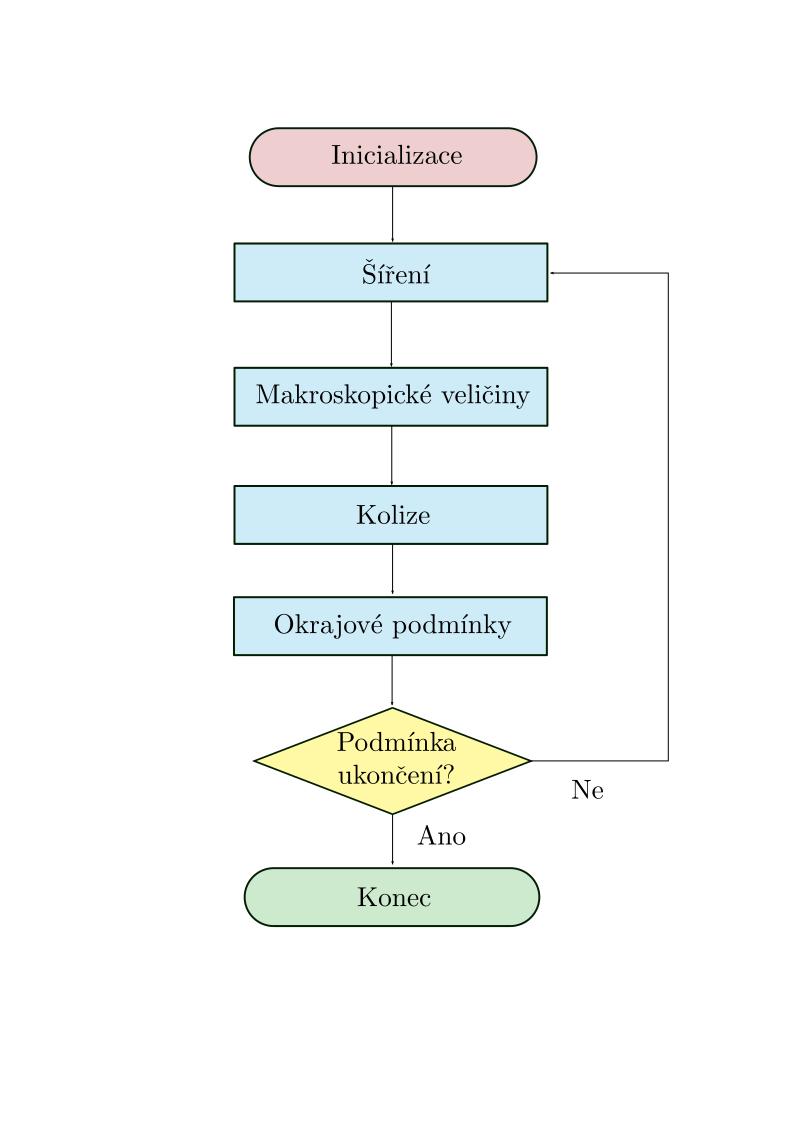
\includegraphics[width=0.3\textwidth]{Images/algoritmus.pdf}
	\caption{Vývojový diagram algoritmu LBM.}
	\label{fig:algo}
\end{figure}


\section{Kolizní operátory}\label{kol}
V diskretizované Boltzmannově transportní \eqref{eq:BTRdiscrete} rovnici vystupuje diskrétní kolizní operátor $ \mathcal{C}_{k} $, jehož zvolená podoba určuje různé typy LBM. Existuje více možností volby  $ \mathcal{C}_{k} $, můžeme pak rozlišit např. varianty SRT-LBM~\cite{GeierCuLBM}, MRT-LBM~\cite{MRT}, CLBM~ \cite{GeierCLBM}, ELBM~\cite{ELBM} nebo CuLBM~\cite{GeierCuLBM}. V této práci se omezíme pouze na využití typu kaskádové LBM (CLBM), který stručně popíšeme v rámci námi uvažovaného rychlostního modelu D2Q9. Detailní odvození metody CLBM lze najít např. v \cite{GeierCLBM}.

Definujme nejdříve diskrétní centrální momenty jako
\begin{equation}\label{eq:centralmoment} 
%\kappa_{(\alpha_{1}, \alpha_{2})} = 
\sum_{k=0}^{8} f_{k} (\xi_{k,1}  - u_{1})^{\alpha_{1}} (\xi_{k,2}  - u_{2})^{\alpha_{2}},
\end{equation}
kde $ \vec{\alpha} = (\alpha_{1}, \alpha_{2}) \in \mathbb{N}^2_{0}$.
%
%Za předpokladu $ \vec{g} = \vec{0}$ zjevně platí
%\begin{subequations}\label{eq:central moments}
%	\begin{eqnarray}
%	k_{(0,0)} &=& \rho,\\[3pt]
%	k_{(1,0)} &=& \sum_{k=0}^{8} f_{k} (\xi_{k,1} - u_{1}) = 0,\\[3pt]
%	k_{(0,1)} &=& \sum_{k=0}^{8} f_{k} (\xi_{k,2} - u_{2}) = 0.
%	\end{eqnarray}
%\end{subequations}

Důležitým aspektem CLBM je, že kolizní krok zmíněný v sekci \ref{algoritmus LBM} je v rámci této metody realizován v prostoru diskrétních centrálních momentů distribučních funkcí, což zlepšuje numerickou stabilitu tohoto schématu \cite{GeierCLBM}. Kolizní operátor CLBM je konstruovaný tak, že každý z centrálních momentů spěje do rovnovážného stavu nezávisle na ostatních centrálních momentech. CLBM využívá při použití rychlostního modelu D2Q9 devět relaxačních parametrů, které označíme jako $ \tau_{0}, \dots, \tau_{8} $ \cite{DP-PE}. 

Matici přechodu z prostoru distribučních funkcí do prostoru momentů označíme $ \mathbf{K} $. Konkrétní tvar báze prostoru momentů distribučních funkcí a matice $ \mathbf{K} $ lze najít např. v \cite{DP-PE}. Podotkněme, že z volby báze toho prostoru se pak odvíjí i tvar transformační matice $ \mathbf{K} $. Jak bylo zmíněno, ke kolizi dochází v rámci schématu CLBM v prostoru centrálních momentů, diskrétní kolizní operátor tedy můžeme psát ve tvaru
\begin{equation}\label{eq:clbm collision}
	\mathcal{C}_k = (\mathbf{K} \vec{v})_k, \ k \in \{0, \dots, 8 \},
\end{equation}
kde pro jednoznačné určení kolize musí být určen tvar $ \vec{v} = (v_0, \dots, v_8)$. Z tvaru matice $ \mathbf{K} $ lze ukázat, že první tři centrální momenty odpovídají hustotě a složkám hybnosti. Hybnost a složky rychlosti se však vlivem kolize nemění, z toho důvodu je tedy pro jednoznačné určení kolize nutné určit pouze složky $ v_3, \dots, v_8 $ a zbylé složky můžeme volit nulové. Odvození tvaru $ v_3, \dots, v_8 $	 lze najít např. v \cite{GeierCLBM, DP-PE}. Dále je nutné určit tvar diskrétního operátoru zdrojových členů $ \mathcal{S}_k, \, k \in \{ 0, \dots, 8\} $ - odvození lze opět najít např. v \cite{GeierCLBM, DP-PE}.


%S pomocí těchto relaxačních časů definujeme diagonální matici 
%\begin{equation}\label{eq:matrixS}
%\mathbf{S} = \mathrm{diag} \, \Bigg( \frac{\Delta t}{\tau_{0}}, \frac{\Delta t}{\tau_{1}}, \dots, \frac{\Delta t}{\tau_{8}} \Bigg)
%\end{equation}
%a vektor $ \vec{f} = \left(f_{0}, f_{1}, \dots, f_{8} \right)^T$  \cite{GeierCLBM}. Kolizní operátor má pak tvar
%\begin{equation}\label{eq:collision operator Ck}
% \mathcal{C}_{k} = \mathbf{K^{-1}}\mathbf{S}(\vec{\kappa}^{\mathrm{eq}} - \vec{\kappa}),
%\end{equation}
%kde $ \mathbf{K} $ je matice přechodu z prostoru distribučních funkcí do prostoru centrálních momentů, $ \vec{\kappa} $ je vektor centrálních momentů splňující $ \vec{\kappa} =  \mathbf{K} \vec{f} $ a $ \vec{\kappa}^{\mathrm{eq}} $ je vektor představující rovnovážné centrální momenty distribučních funkcí \cite{GeierCLBM}. Matici přechodu $ \mathbf{K} $ volíme tak, aby vektor $ \vec{\kappa} $ splňoval
%\begin{equation}\label{eq:kappa}
%\vec{\kappa} = (k_{(0,0)}, k_{(1,0)}, k_{(0,1)}, k_{(1,1)}, k_{(2,0)} + k_{(0,2)}, k_{(2,0)} - k_{(0,2)}, k_{(2,1)}, k_{(1,2)} , k_{(2,2)})^T,
%\end{equation}
%a aby platilo
%\begin{equation}\label{eq:kappaeq}
%\vec{\kappa}^{\mathrm{eq}} = (\rho, 0, 0, 0, 2 \rho c^{2}_{s}, 0, 0, 0, \rho c^{4}_{s})^T.
%\end{equation}
Prozkoumejme dále tvar relaxačních parametů $ \tau_{0}, \dots, \tau_{8}$. Platí, že $ \nu $ je závislá na relaxačních parametrech $ \tau_{4} $ a $ \tau_{5} $. S využitím předpokladu izotropie viskozity \cite{DP-PE} můžeme volit
\begin{equation}
\tau_{4} = \tau_{5} = \tau,
\end{equation}
kde hodnota $ \tau $ splňuje
\begin{equation}\label{eq:tauclbm}
\nu = c^{2}_{s} \, \Bigg( \tau  - \frac{\Delta t}{2} \Bigg).
\end{equation}
Další relaxační parametry lze volit ke zlepšení numerické stability a volíme je dle \cite{GeierCLBM} jako
\begin{equation}
\tau_{3} = \tau_{6} = \tau_{7} = \tau_{8} = 1,
\end{equation}
přičemž na hodnotách $ \tau_{0}, \tau_{1} $ a $ \tau_{2} $ z důvodu tvaru složek vektoru $\vec{v}$ nezáleží.

\section{Počáteční a okrajové podmínky}\label{pocatecni a okrajove podminky}

Vhodná volba počátečních a okrajových podmínek, která je v souladu se zkoumanou úlohou, je nedílnou součástí následné numerické simulace. Z důvodu specifického mezoskopického popisu tekutiny v rámci LBM je volbě počátečních a okrajových podmínek později použitých v praktické části práce nutné věnovat zvýšenou pozoronost, a proto jsou dále použité počáteční a okrajové podmínky podrobněji popsány.

\subsection{Počáteční podmínka}\label{pocatecni podminka}
Uvažujme nyní oblast definovanou vztahy \eqref{eq:oblast}. K nastavení počáteční podmínky využijeme rovnovážnou distribuční funkci $ f^{\mathrm{eq}} $, která má tvar 
\begin{equation}\label{eq:feq}
f^{\mathrm{eq}}_{k} = \rho w_{k} \, \Bigg(1 + \frac{\vec{\xi_{k}} \cdot \vec{u}}{c^{2}_{s}} + \frac{(\vec{\xi_{k}} \cdot \vec{u})^2}{2c^{4}_{s}} - \frac{\vec{u} \cdot \vec{u}}{2c^{2}_{s}} \Bigg)\, , \hspace{2mm} k \in \{0,\dots,q-1\},
\end{equation}
kde $ w_{k} $ představují váhy specifické pro vybraný rychlostní model, přičemž pro použitý model D2Q9 platí~\cite{Kruger}
\begin{align}\label{weighs}
\begin{split}
w_{0} &  = \dfrac{4}{9},\\[4pt]
w_{1} = w_{2} = w_{3} = w_{4} & = \frac{1}{9},\\[4pt]
w_{5} = w_{6} = w_{7} = w_{8} & = \frac{1}{36}.
\end{split}
\end{align}
Počáteční rozložení $ \rho $, resp. $ \vec{u} $, definujeme jako $ \rho _{\mathrm{ini}} $, resp. $ \vec{u} _{\mathrm{ini}} $. Poté pro každý uzel $ \vec{x} \in \hat{\Omega} $ v čase $ t=0 $ bude platit

\begin{equation}\label{eq:initial condition}
f^{}_{k} (\vec{x}, 0) = f^{\mathrm{eq}}_{k} (\rho _{\mathrm{ini}} (\vec{x}), \vec{u} _{\mathrm{ini}} (\vec{x})), \hspace{3mm} k \in \{0, 1, \dots q-1\}.
\end{equation}
V rámci tohoto přístupu nastavení počáteční podmínky předpokládáme, že nerovnovážná část distribučních funkcí $ f^{\mathrm{neq}}_{k} = f_{k} - f^{\mathrm{eq}}_{k}$ může být zanedbána a distribuční funkce mohou tak být aproximovány svou rovnovážnou částí. Značnou výhodou této volby aproximace počáteční podmínky je její následná jednoduchá implementace, a proto je v rámci této práce použita, byť existují i jiné, sofistikovanější, volby, viz např. \cite{PE}.

\subsection{Okrajové podímky}


\subsubsection{Bounce-back okrajová podmínka}\label{bounce-back}
První zmíněnou okrajovou podmínkou je bounce-back okrajová podmínka, konkrétně její varianta \textit{fullway}. Bounce-back okrajová podmínka se typicky používá na rozhraní tekutiny a pevné látky. Její výhoda je, že na rozhraní splňuje neklouzavou (anglicky \textit{no-slip}) okrajovou podmínku a že její implementace je přímočará. Princip bounce-back okrajové podmínky je takový, že na rozhraní dojde k myšlenému odrazu distribučních funkcí odpovídajích částicím s mikroskopickou rychlostí $ \vec{\xi_{k}} $ zpět do směrů, ze kterých se do daného uzlu dostaly s rychlostí $ \vec{\xi_{\bar{k}}} = -\vec{\xi_{k}}$.

Při použití této okrajové podmínky se rozhraní nachází v polovině vzdálenosti mezi uzly tekutiny a tělesa. Tato skutečnost nepůsobí problémy při modelování proudění okolo rovných zdí, které jsou rovnoběžné s použitou mřížkou. Pro zakřivené hranice nerovnoběžné s mřížkou však metoda bounce-back dává za vznik "schodovitému" \ tvaru hranice, a tedy neposkytuje vhodnou aproximaci skutečné pozice rozhraní, viz obr. \ref{fig:staircase}.

\begin{figure}[H]
	\centering
	\vspace{2mm}
	\includegraphics[width=0.37\textwidth]{Images/stairboundary.pdf}
	\vspace{2mm}
	\caption{"Schodovitý" \ tvar hranice vznikající při použití bounce-back okrajové podmínky.}
	\label{fig:staircase}
	\vspace{1.8mm}
\end{figure}


Fullway varianta bounce-back okrajové podmínky vyžaduje ke své realizaci a odražení hypotetických částic dva časové kroky. Během nich doputují částice až do uzlů pevné látky, kde je jejich směr následně v dalším kroku šíření obrácen, jak je schematicky znázorněno na obr. \ref{fig:bb}.

\begin{figure}[h]
	\centering
	\vspace{2mm}
	\hspace{7mm}
	\includegraphics[width=0.9\textwidth]{Images/bb.pdf}
	\vspace{2.8mm}
	\caption{Schématické znázornění fullway bounce-back okrajové podmínky. Šipky představují směr šíření hypotetické částice, oblast s šedou barvou představuje pevné těleso a čárkovaná hranice odpovídá pozici rozhraní.}
	\label{fig:bb}
	\vspace{1.8mm}
\end{figure}


Podotkněme, že dále existuje \textit{halfway} varianta bounce-back okrajové podmínky, která ke své realizaci potřebuje pouze jeden časový krok, detaily lze najít např. v \cite{Kruger}. Nicméně v rámci této práce se omezíme pouze na využití varianty fullway.
 

\subsubsection{Interpolační okrajové podmínky}\label{interpolation bc}
Jak již bylo zmíněno, bounce-back okrajová podmínka nereflektuje správným způsobem zakřivenou hranici tělesa. Vhodnější volbou okrajové podmínky pro rozhraní tekutiny a tělesa se zakřivenou hranicí jsou tzv. interpolační okrajové podmínky.

Obě dále zmíněné interpolační okrajové podmínky využívají k výpočtu distribučních funkcí lineární nebo kvadratickou interpolaci, při níž je použit bezrozměrný parametr $ \Theta $ definovaný vztahem
\begin{equation}\label{eq:q}
\Theta = \frac{\norm{\vec{x}_{f{_A}}-\vec{x}_w}}{\norm{\vec{x}_{f{_A}}-\vec{x}_b}},
\end{equation}
kde $ \vec{x}_{f{_A}} $ je uzel tekutiny na hranici, $ \vec{x}_b =  \vec{x}_{f{_A}} + \Delta t \vec{\xi_{k}}$ je uzel pevné překážky, dále $ \vec{x}_w$ se nachází na skutečné hranici objektu tak, jak je ilustrováno na obr. \ref{fig:bouz}. Pro pozdější využití navíc dále zavádíme body \mbox{$ \vec{x}_{f{_B}} = \vec{x}_{f{_A}} + \Delta t \vec{\xi_{\bar{k}}} \,$} a $\,  \vec{x}_{f{_C}} = \vec{x}_{f{_A}} + 2\Delta t \vec{\xi_{\bar{k}}}  $, kde index $ \bar{k} $ splňuje $ \vec{\xi_{\bar{k}}} = -\vec{\xi_{k}}$. Jejich význam je společně s významem vzdáleností použitých ve výpočtu parametru $ \Theta $ znázorněn na obr. \ref{fig:bouz2}. Podotkněme, že na hranici tělesa dále uvažujeme no-slip podmínku.
\begin{figure}[H]
	\centering
	\begin{subfigure}{0.95\textwidth}
		\centering
		\includegraphics[width=0.45\textwidth]{Images/bouzidi.pdf}
		\caption{Ilustrace významu bodů $ \vec{x}_{f{_A}}, \vec{x}_w, \vec{x}_b$. Černé body na skutečné hranici tělesa představují pozice všech bodů $ \vec{x}_w$, které slouží k výpočtu parametru $ \Theta $ pro různé body tekutiny $ \vec{x}_{f{_A}} $ pro různé směry.}
		\label{fig:bouz}
	\end{subfigure}%
	\\[10pt]
	\begin{subfigure}{0.95\textwidth}
		\centering
		\includegraphics[width=0.85\textwidth]{Images/bouzidi2.pdf}
		\caption{Ilustrace významu bodů $ \vec{x}_{f{_B}} $ a $ \vec{x}_{f{_C}} $ a vzdáleností vyskytujících se ve výpočtu parametru $ \Theta $.}
		\label{fig:bouz2}
	\end{subfigure}
	\vspace{3mm}
	\caption{Schématické znázornění významu členů využitých v rámci interpolačních okrajových podmínek. Šedá oblast představuje oblast tělesa.}
	\label{fig:lattice}
\end{figure}

Jako první představíme interpolační okrajovou podmínku navrženou M. Bouzidim a kol. (dále jen Bouzidiho okrajová podmínka) v \cite{Bouzidi2001}. Popíšeme proces využitý k odvození jejího tvaru při lineární interpolaci.

Uvažujme nejdříve $ \Theta \geq \frac{1}{2} $, tedy případ, kdy se skutečná hranice nachází blíže bodu $ \vec{x}_b $. Myšlená částice v $ \vec{x}_{f{_A}} $ pohybující se s rychlostí $ \vec{\xi_{k}} $ v čase $ t $ se od stěny odrazí v čase $ t + \Theta \Delta t$ v hraničním bodě $ \vec{x}_w $ s opačnou rychlostí $ \vec{\xi_{\bar{k}}} $. Po uplynutí dalšího časového úseku $ (1 - \Theta ) \Delta t $, tj. v čase $ t + \Delta t$ se částice bude nacházet v~bodě $ \vec{x}_t $, pro který platí
\begin{equation}
	\vec{x}_t = \vec{x}_f + (2\Theta - 1)\Delta t \vec{\xi}_{k}.
\end{equation}
Platí tedy $ f_{\bar{k}} (\vec{x}_t, t + \Delta t) = f^{*}_k ( \vec{x}_{f{_A}}, t)$. Schéma tohoto odrazu je k nahlédnutí na obr. \ref{fig:interp1}. Hodnota $ f_{\bar{k}} (\vec{x}_t, t + \Delta t)$ společně se známou hodnotou $ f_{\bar{k}} ( \vec{x}_{f{_B}}, t) = f^{*}_{\bar{k}} ( \vec{x}_{f{_A}}, t)$ je pak lineárně interpolována a tím je získána hodnota $ f_{\bar{k}}\left(\vec{x}_{f{_A}}, t+\Delta t\right) $.

Dále uvažejme $ \Theta < \frac{1}{2} $, tedy případ, kdy se skutečná hranice nachází blíže bodu $ \vec{x}_{f_A} $. Pro interpolaci využijeme bod
\begin{equation}
\vec{x}_t = \vec{x}_f + (1 - 2\Theta)\Delta t \vec{\xi}_{\bar{k}}.
\end{equation}
Myšlená částice v $ \vec{x}_{t} $ pohybující se s rychlostí $ \vec{\xi_{k}} $ v čase $ t $ se od stěny odrazí v čase $ t + (1 - \Theta) \Delta t$ v bodě $ \vec{x}_w $ s opačnou rychlostí $ \vec{\xi_{\bar{k}}} $. Za další časový úsek $ \Theta \Delta t $ se bude vyskytovat v bodě $ \vec{x}_{f{_A}} $. Platí tedy $ f^{*}_{k} (\vec{x}_t, t) = f_{\bar{k}} (\vec{x}_{f{_A}}, t + \Delta t)$. Schéma tohoto odrazu je k nahlédnutí na obr. \ref{fig:interp2}. Hodnotu $ f^{*}_{k} (\vec{x}_t, t) $ získáme lineární interpolací hodnot $ f^{*}_{k} (\vec{x}_{f_A}, t) $ a $ f^{*}_{k} (\vec{x}_{f_B}, t) $.
\begin{figure}[H]
	\centering
	\begin{subfigure}{0.5\textwidth}
		\centering
		\includegraphics[width=0.95\textwidth]{Images/interpolace1.pdf}
		\vspace{2mm}
		\caption{Ilustrace odrazu částice při hodnotě $ \Theta \geq \frac{1}{2} $.}
		\label{fig:interp1}
	\end{subfigure}%
	\begin{subfigure}{0.5\textwidth}
		\centering
		\includegraphics[width=0.95\textwidth]{Images/interpolace2.pdf}
		\vspace{2mm}
		\caption{Ilustrace odrazu částice při hodnotě $ \Theta < \frac{1}{2} $.}
		\label{fig:interp2}
	\end{subfigure}
	\caption{Schématické znázornění konstrukce použité při odvození Bouzidiho okrajové podmínky za použití lineární interpolace.}
	\label{fig:interp}
\end{figure}

Shrneme-li výsledky lineární interpolace pro oba zmínené případy hodnoty parametru $ \Theta $, má Bouzidiho okrajová podmínka tvar
\begin{align}\label{eq:lbouz}
\begin{split}
\Theta &< \dfrac{1}{2}: \hspace{7mm} 
f_{\bar{k}}\left(\vec{x}_{f{_A}}, t+\Delta t\right) = 2 \Theta f_{k}^{*}\left(\vec{x}_{f{_A}}, t\right)+(1-2 \Theta) f_{k}^{*}\left(\vec{x}_{f{_B}}, t\right),\\[6pt]
\Theta &\geq \dfrac{1}{2}: \hspace{7mm} f_{\bar{k}}\left(\vec{x}_{f{_A}}, t+\Delta t\right) = \frac{1}{2 \Theta} f_{k}^{*}\left(\vec{x}_{f{_A}}, t\right)+\frac{2 \Theta-1}{2 \Theta} f_{\bar{k}}^{*}\left(\vec{x}_{f{_A}}, t\right).
\end{split}
\end{align}

Jak bylo zmíněno, k odvození lze použít i kvadratickou interpolaci. Při použití kvadratické interpolace má Bouzidiho okrajová podmínka tvar
\begin{align}\label{eq:qbouz}
\begin{split}
\Theta &< \dfrac{1}{2}: \hspace{3mm} 
f_{\bar{k}}\left(\vec{x}_{f{_A}}, t+\Delta t\right) =
\Theta \left( 1 + 2\Theta \right) f_{k}^{*}\left(\vec{x}_{f{_A}}, t\right)+
(1-4 \Theta^2) f_{k}^{*}\left(\vec{x}_{f{_B}}, t\right)-
\Theta \left( 1 - 2\Theta \right) f_{k}^{*}\left(\vec{x}_{f{_C}}, t\right),\\[6pt]
\Theta &\geq \dfrac{1}{2}: \hspace{3mm}
f_{\bar{k}}\left(\vec{x}_{f{_A}}, t+\Delta t\right) =
\frac{1}{\Theta \left(2 \Theta + 1\right)} f_{k}^{*}\left(\vec{x}_{f{_A}}, t\right) +
\frac{2\Theta - 1}{\Theta} f_{\bar{k}}^{*}\left(\vec{x}_{f{_A}}, t\right) -
\frac{2\Theta - 1}{2 \Theta + 1} f_{\bar{k}}^{*}\left(\vec{x}_{f{_B}}, t\right).
\end{split}
\end{align}

Bouzidiho interpolační schéma používá dva různé vzorce na základě hodnoty parametru $ \Theta $. V~\cite{Yu2003}~však bylo odvozeno interpolační schéma, které oba případy sjednocuje v jeden společný tvar pro všechny hodnoty~$ \Theta $. Okrajovou podmínku využívající toto schéma nazýváme sjednocená okrajová podmínka (anglicky \textit{unified interpolation scheme}). Opět lze pro její odvození využít lineární nebo kvadratickou interpolaci.
Při použití lineární interpolace má sjednocená okrajová podmínka tvar
\begin{equation}\label{eq:luni}
f_{\bar{k}}\left(\vec{x}_{f{_A}}, t+\Delta t\right)= \frac{1}{1+\Theta} \, \Big[ \Theta f_{k}\left(\vec{x}_{f{_A}}, t\right)+(1-\Theta) {f}_{k}\left(\vec{x}_{f{_B}}, t\right) +\Theta {f}_{\bar{k}}\left(\vec{x}_{f{_A}}, t\right) \Big].
\end{equation}
Použitím kvadratické interpolace získáme pro sjednocenou okrajovou podmínku tvar
\begin{align}\label{eq:quni}
\begin{split}
f_{\bar{k}}\left(\vec{x}_{f_A}, t+\Delta t\right)=& \,
\frac{1}{(1+\Theta)(2+\Theta)} \, \Big[\Theta(1+\Theta) {f}_{k}\left(\vec{x}_{f{_A}}, t\right)+2\left(1-\Theta^{2}\right) {f}_{k}\left(\vec{x}_{f{_B}}, t\right)
\\&-\Theta(1-\Theta) {f}_{k}\left(\vec{x}_{f{_C}}, t\right)+2 \Theta(2+\Theta) {f}_{\bar{k}}\left(\vec{x}_{f{_A}}, t\right) 
-\Theta(1+\Theta) {f}_{\bar{k}}\left(\vec{x}_{f{_B}}, t\right) \Big].
\end{split}\end{align}

\subsubsection{Rovnovážná okrajová podmínka}\label{equilibrium bc}
Jednou z možností jak aproximovat neznáme hodnoty distribučních funkcí v krajních uzlových bodech oblasti je pomocí rovnovážné distribuční funkce jako \cite{PE}

\begin{equation}
	f_i(\vec{x}, t)=f_{i}^{\text{(eq)}}(\rho(\vec{x}, t), \vec{u}(\vec{x}, t)), \hspace{2mm}  \forall k \in \{0,\dots,q-1\}, \forall t \in \hat{\mathcal{I}}.
\end{equation}

Výhodou této aproximace je její snadná implementace, nevýhodou je zanedbání nerovnovážné části distribuční funkce \cite{PE}.

\subsubsection{Momentová okrajová podmínka}\label{moment based bc}

Momentová okrajová podmínka (anglicky \textit{moment-based boundary condition}) představuje způsob, jak na hranicích oblasti předepsat okrajovou podmínku na základě znalosti příslušných makroskopických momentů, s pomocí nichž a známých hodnot distribučních funkcí jsou zbylé, neznámé, distribuční funkce jednoznačně vyjádřitelné. Detaily odvození této okrajové podmínky lze najít v \cite{PE}.

Při použití momentové okrajové podmínky je předpokládána znalost diskrétních obecných momentů definovaných jako
\begin{equation}\label{eq:raw moments}
m_{(\alpha_{1}, \alpha_{2})} = \sum_{k=0}^{q-1} f_{k} \xi^{\alpha_{1}}_{k,1} \xi^{\alpha_{2}}_{k,2},
\end{equation}
kde $ \vec{\alpha} = (\alpha_{1}, \alpha_{2}) \in \mathbb{N}^2_{0}$.

Podobně jako tomu bylo pro centrální momenty v sekci \ref{kol}, lze zavést matici přechodu z prostoru distribučních funkcí do prostoru obecných momentů. Tuto matici budeme značit $ \mathbf{M} $, její konkrétní podobu lze najít např. v \cite{LBMAT}. Jelikož je $ \mathbf{M} $ regulární, lze na základě obecných momentů a známých hodnot distribučních funkcí vyjádřit libovolný počet neznámých distribučních funkcí. Pro výpočet hustoty lze využít hodnot známých distribučních funkcí a zadané rychlosti, naopak pro výpočet rychlosti použijeme známe distribuční funkce a zadanou hustotu.

Podotkněme, že z charakteru momentové okrajové podmínky vyplývá, že vztahy pro výpočet neznámých distribučních funkcí musí být odvozeny zvlášť pro každou požadovanou množinu těchto neznámých - v rámci modelu D2Q9 to znamená odvození pro 4 různé strany obdélníkové oblasti a 4 zbývající navzájem různé rohy této oblasti. Konkrétní vztahy pro každou tuto neznámou množinu distribučních funkcí 
%jsou k nahlédnutí v \cite{PE}.
jsou pro úplnost k nahlédnutí v příloze~\ref{priloha A}.


\section{Výpočet síly v LBM}\label{vypocet sily v LBM}

Existují dva standardní způsoby výpočtu síly v rámci LBM - metoda výměny hybnosti a metoda integrace tenzoru napětí, viz \cite{NASA}. Zde popíšeme pouze metodu integrace tenzoru napětí, detaily ohledně metody výměny hybnosti lze najít např. v \cite{NASA}. Dále uvažujme oblast~$ \Omega $, těleso $ \Omega_{\mathrm{b}} \subset \Omega $ a zkoumejme sílu, kterou tekutina v oblasti působí na těleso.

Metoda integrace tenzoru napětí (anglicky \textit{stress integration method}) je přímo založena na vztahu~\eqref{eq:stress_int}. Zapíšeme-li tento vztah v diskrétním tvaru, integrál přejde v sumu přes konečný počet bodů a~pro $ i $-tou složku síly $ \vec{F} $ dostaneme vztah ve tvaru
\begin{equation}\label{eq:sim}
{F}_{i}(t) = \sum_{\vec{x} \in  \partial \hat{\Omega}_{\mathrm{b}}}^{} \Delta s(\vec{x}) \sum_{j=1}^{2}  \sigma_{ij} (\vec{x}, t) \, n_{j} (\vec{x})  , \hspace{2mm} i \in \{ 1, 2 \},
\end{equation}
kde $ \Delta s(\vec{x}) $ \si{[-]} představuje bezrozměrnou náhradu diferenciálu $ \mathrm{d}S $ (viz~\eqref{eq:stress_int}) v bodě $ \vec{x}$, $ \sigma_{ij} (\vec{x}, t)$ představuje složky diskrétního úplného tenzoru napětí v bodě $ \vec{x} $ a v čase $ t $, dále pak $ \vec{n}(\vec{x}) $ představuje jednotkový vnější normálový vektor hranice tělesa v bodě $ \vec{x} \in \partial \hat{\Omega}_{\mathrm{b}}$. Upozorněme, že body z $ \partial \hat{\Omega}_{\mathrm{b}} $, tj. body diskretizující hranici obtékaného tělesa, se nemusí obecně nacházet na diskrétní mřížce $ \hat{\Omega} $, a tedy musí být hodnota tenzoru napětí v těchto bodech extrapolována z okolních bodů mřížky. Obecně totiž hranici obtékaného tělesa parametrizujeme množinou lagrangeovských bodů, které, jak bylo zmíněno, nemusí nutně ležet v $ \hat{\Omega} $. Vztah bodů diskretizujících hranici obtékaného tělesa a uzlů mřížky je schematicky znázorněn na obr. \ref{fig:body hranice sim}. Popis hranice objektů je podrobněji rozebrán v kapitole \ref{geometrie}.

K výpočtu hodnoty $ \sigma_{ij} $ v bodech mřížky lze využít aproximace pomocí konečných diferencí nebo explicitní vztahy pro lokální výpočet, jak bylo zkoumáno v předchozí bakalářské práci \cite{JB}.

\begin{figure}[H]
	\centering
	\includegraphics[width=0.32\textwidth]{Images/stressintegration.pdf}
	\caption{Schématické znázornění rozdílu mezi uzly mřížky a body diskretizujícími hranici obtékaného tělesa, které jsou vyznačeny černou barvou.}
	\label{fig:body hranice sim}
\end{figure}


\section{Poznámky k implementaci LBM}\label{poznamky k implementaci LBM}
Jak již bylo zmíněno v úvodu práce, pro numerické řešení pomocí LBM byl využit kód vyvíjený na katedře matematiky (dále jen KM) FJFI ČVUT v Praze, který slouží k řešení Navierových-Stokesových rovnic pro newtonovskou nestlačitelnou tekutinu. Program je implementovaný v jazyce C++ a využívá paralelizace na GPU s využitím platformy CUDA. V kódu je pro model D2Q9 implementována použitá varianta mřížkové Boltzmannovy metody CLBM.

Pro účely této práce byl rozšířen kód vzniklý v rámci předchozí bakalářské práce \cite{JB}, v kterém byla oproti vyvíjenému kódu na KM FJFI  provedena řada úprav, zejména:
\begin{itemize}
	\item implementace metody integrace tenzoru napětí pro výpočet síly pomocí diference,
	\item implementace různých způsobů lokálního výpočtu tenzoru napětí,
	\item implementace interpolačních okrajových podmínek,
	\item výpočet sledovaných veličin a jejich následný výpis do souborů.
\end{itemize}
V kódu byl pak v rámci této práce implementován výpočet zkoumaných účelových funkcí a také momentová okrajová podmínka. Pro implementaci momentové okrajové podmínky pro model D2Q9 byl využit generátor vytvořený Ing. Pavlem Eichlerem implementovaný v C++ využívající knihovnu GiNaC \cite{Ginac}, umožňující provádět symbolické matematické operace.
